% !TeX root = ../main.tex
\subsection{问题三：多工序生产的期望递推与精确枚举}

根据题目给出的两级装配关系，将生产系统表示为
\begin{equation}
  \{1,2,3\}\to H_1,\qquad
  \{4,5,6\}\to H_2,\qquad
  \{7,8\}\to H_3,\qquad
  \{H_1,H_2,H_3\}\to F.
  \label{eq:q3-structure}
\end{equation}
与问题二不同，本问不继续求解信息状态自适应策略，而把各环节检测/拆解决策限制为生产前预先确定的固定 0-1 策略；该策略类限制使 16 个决策变量的空间可以精确遍历，是问题二方法在大规模结构下的明确简化。

\subsubsection{任务、生产结构与决策变量}

本题需要确定 8 个零配件是否检测、3 个半成品是否检测、不合格半成品是否拆解、成品是否检测以及不合格成品是否拆解。表~\ref{tab:q3-params}给出该情形的全部参数：零配件、半成品与成品次品率均为 $10\%$，市场售价为 $200$ 元，调换损失为 $40$ 元。

\begin{table}[H]
  \centering
  \caption{问题三的生产与成本参数（单位：元/件）}
  \label{tab:q3-params}
  \small
  \begin{tabular}{lcccccc}
    \toprule
    对象 & 次品率 & 购买单价 & 检测成本 & 装配成本 & 拆解费用 & 其他 \\
    \midrule
    零配件 1 & $10\%$ & $2$ & $1$ & --- & --- & --- \\
    零配件 2 & $10\%$ & $8$ & $1$ & --- & --- & --- \\
    零配件 3 & $10\%$ & $12$ & $2$ & --- & --- & --- \\
    零配件 4 & $10\%$ & $2$ & $1$ & --- & --- & --- \\
    零配件 5 & $10\%$ & $8$ & $1$ & --- & --- & --- \\
    零配件 6 & $10\%$ & $12$ & $2$ & --- & --- & --- \\
    零配件 7 & $10\%$ & $8$ & $1$ & --- & --- & --- \\
    零配件 8 & $10\%$ & $12$ & $2$ & --- & --- & --- \\
    半成品 1--3 & $10\%$ & --- & $4$ & $8$ & $6$ & --- \\
    成品 & $10\%$ & --- & $6$ & $8$ & $10$ & 售价 $200$，调换损失 $40$ \\
    \bottomrule
  \end{tabular}
\end{table}

把全部决策编码为 16 位二元向量
\begin{equation}
  X=(x_1,\ldots,x_{16}),\qquad x_i\in\{0,1\},
  \label{eq:q3-strategy}
\end{equation}
其中 $x_1$--$x_8$ 表示零配件 1--8 是否检测，$x_9$--$x_{11}$ 表示半成品 1--3 是否检测，$x_{12}$--$x_{14}$ 表示检测出的不合格半成品 1--3 是否拆解，$x_{15}$ 表示成品是否检测，$x_{16}$ 表示不合格成品是否拆解；取值 $1$ 表示检测或拆解，$0$ 表示不检测或不拆解。搜索空间大小为 $2^{16}=65536$。图~\ref{fig:q3-structure}给出该情形的装配结构与决策位示意。

\begin{figure}[!htbp]
  \centering
  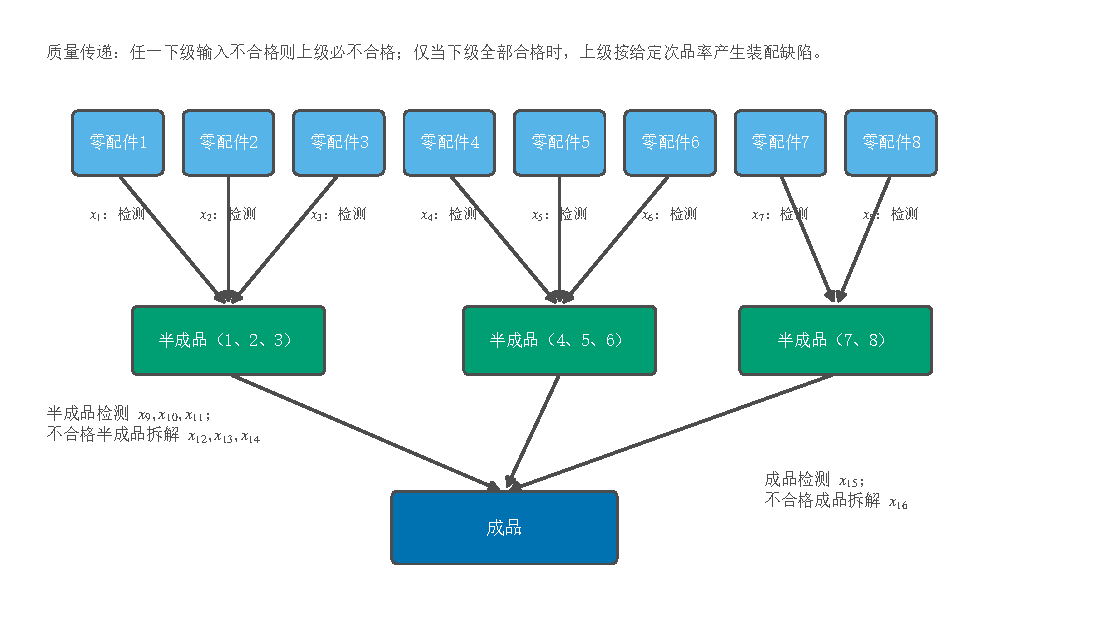
\includegraphics[width=0.95\textwidth]{../../figures/q3/fig_q3_structure.pdf}
  \caption{问题三的两工序生产结构与 16 位决策变量}
  \label{fig:q3-structure}
\end{figure}

\subsubsection{质量状态与传递规则}

对每个零配件和半成品维护四态
\begin{equation}
  s\in\{N,KG,UG,UB\},
  \label{eq:q3-state}
\end{equation}
其中 $N$ 表示当前没有该对象，$KG$ 表示已知合格，$UG$ 与 $UB$ 分别表示未检测但实际合格与实际不合格。系统状态记为
\begin{equation}
  S=(s_1,\ldots,s_8,h_1,h_2,h_3),
  \label{eq:q3-system-state}
\end{equation}
初始状态为 $S_0=(N,\ldots,N)$。状态必须满足装配层级一致性：当半成品 $H_j$ 已完成装配时，其下级零配件不再作为独立在手对象参与后续装配，仅在 $H_j$ 被拆解后才重新显式恢复下级状态；因此程序只生成满足该一致性的可达状态，而不是 $4^{11}$ 个形式组合。

质量沿装配层级传递，规则为：

\begin{enumerate}
  \item 零配件没有主动报废或拆解决策；若检测，则丢弃检测出的不合格件并重复购检直至合格件进入装配，若未检测则直接进入装配；
  \item 拆解决策只作用于不合格半成品或不合格成品；拆解不损坏内部下级零部件，回流后保留原真实质量状态，不重新按次品率抽样；
  \item 若任一下级输入不合格，则上级产品必为不合格；
  \item 仅当全部下级输入合格时，上级产品才以给定次品率产生装配缺陷。
\end{enumerate}

\subsubsection{固定策略的期望成本递推}

设 $S_T$ 表示成功交付一件合格成品的吸收状态，约定 $V_X(S_T)=0$。对固定策略 $X$，$V_X(S)$ 表示从状态 $S$ 出发最终交付的期望成本。零配件 $i$ 若选择检测，则由几何分布的期望试验次数，购检并得到合格件的期望成本为
\begin{equation}
  C_i^{T}=\frac{c_i+t_i}{1-p_i},
  \label{eq:q3-buy-test}
\end{equation}
其中 $c_i$、$t_i$、$p_i$ 分别为购买单价、检测成本与次品率；若不检测，成本为 $C_i^{N}=c_i$，并以概率 $1-p_i$ 与 $p_i$ 分别进入 $UG$ 与 $UB$ 状态。

设半成品 $H_j$ 的下级零配件集合为 $G_j$。若所有下级零配件实际合格，则
\begin{equation}
  P(H_j\text{ 合格})=1-p_{H_j},\qquad
  P(H_j\text{ 不合格})=p_{H_j};
  \label{eq:q3-semi-quality}
\end{equation}
若存在任一下级零配件不合格，则 $P(H_j\text{ 不合格})=1$。成品装配同理，三个半成品均实际合格时成品合格概率为 $1-p_F$，否则成品必不合格。

以半成品 $H_1$ 的装配与检测为例说明一步成本与转移概率的构造。设当前状态 $S$ 中零件 1--3 已持有且实际均合格，$H_1$ 未装配。装配支付 $a_1$ 后，$H_1$ 以概率 $1-p_{H_1}$ 合格、$p_{H_1}$ 不合格。若 $x_9=0$，一步成本为 $C_X(S)=a_1$，转移为
\begin{equation}
  P_X(S_1\mid S)=1-p_{H_1}\ (h_1\to UG),\qquad
  P_X(S_2\mid S)=p_{H_1}\ (h_1\to UB);
  \label{eq:q3-example-notest}
\end{equation}
若 $x_9=1$，检测支付 $T_1$：检测合格时 $h_1\to KG$，概率 $1-p_{H_1}$，成本 $a_1+T_1$；检测不合格且 $x_{12}=1$ 时再支付拆解费用 $D_1$，$h_1\to N$ 且零件 1--3 按原真实状态回流，概率 $p_{H_1}$，成本 $a_1+T_1+D_1$；检测不合格且 $x_{12}=0$ 时，半成品与下级零件报废并回到对应采购状态，概率 $p_{H_1}$，成本 $a_1+T_1$。其余半成品与成品环节按同一规则递归构造，程序据此为每个策略生成全部可达状态、一步成本与转移概率。

对任意状态 $S$ 建立递推方程
\begin{equation}
  V_X(S)=C_X(S)+\sum_{S'}P_X(S'\mid S)V_X(S'),
  \label{eq:q3-value}
\end{equation}
其中 $P_X$ 是非终止可达状态之间的转移子矩阵：由于部分概率流向吸收状态 $S_T$，$P_X$ 为严格次随机矩阵。将所有非终止状态联立得到
\begin{equation}
  (I-P_X)V_X=C_X.
  \label{eq:q3-linear}
\end{equation}

若从初始状态出发最终以概率 $1$ 到达 $S_T$ 且到达的期望步数有限，则称策略 $X$ 可行；此时谱半径 $\rho(P_X)<1$，$I-P_X$ 可逆，且
\begin{equation}
  V_X=(I-P_X)^{-1}C_X.
  \label{eq:q3-inverse}
\end{equation}
若策略存在不含 $S_T$ 的闭合状态类，则 $\rho(P_X)\ge1$，期望成本无有限解，策略不可行。程序中以线性方程组是否可解等价实现该判据，矩阵求解只是实现方式。初始状态期望成本为 $E[C\mid X]=V_X(S_0)$，期望利润为
\begin{equation}
  E[\Pi(X)]=R-V_X(S_0),
  \label{eq:q3-profit}
\end{equation}
优化目标为
\begin{equation}
  X^\ast=\arg\max_{X\in\{0,1\}^{16}}E[\Pi(X)].
  \label{eq:q3-objective}
\end{equation}

\subsubsection{全策略枚举与精确求解}

本题仅有 16 个二元决策变量，固定策略空间共有 $2^{16}=65536$ 种，仍可精确遍历。因此本文对全部策略进行枚举，并利用 5.3.3 节的期望成本递推逐一评价，获得固定策略空间内的全局最优解；每个策略的线性方程组规模不超过 1122 个状态。

\subsubsection{最优策略与结果分析}

全枚举得到固定策略空间内的最优策略 $1111111111111101$，其含义见表~\ref{tab:q3-optimal}：8 个零配件与 3 个半成品全部检测，不合格半成品全部拆解，成品不检测，不合格成品拆解。最优期望成本为 $139.7778$ 元，最优期望利润为 $60.2222$ 元，对应的可达状态数为 18。

\begin{table}[H]
  \centering
  \caption{最优策略 $1111111111111101$ 的决策含义}
  \label{tab:q3-optimal}
  \begin{tabular}{ll}
    \toprule
    决策位 & 含义 \\
    \midrule
    $x_1$--$x_8=11111111$ & 零配件 1--8 全部检测，检出不合格件丢弃后重复购检 \\
    $x_9$--$x_{11}=111$ & 半成品 1--3 全部检测 \\
    $x_{12}$--$x_{14}=111$ & 检测出的不合格半成品 1--3 全部拆解，零配件回流 \\
    $x_{15}=0$ & 成品不检测，不合格品进入市场后按调换处理 \\
    $x_{16}=1$ & 退回的不合格成品拆解，零配件与半成品回流 \\
    \bottomrule
  \end{tabular}
\end{table}

图~\ref{fig:q3-landscape}给出全部 65536 个策略的期望利润分布。在 65536 个策略中，仅有 17060 个可行，其余 48476 个不可行；可行策略的期望利润均值为 $-33.01$ 元、中位数为 $-29.23$ 元，只有 4310 个策略盈利。利润分布整体偏向负值，最优值 $60.2222$ 元比次优策略高 $2.1728$ 元，高利润决策集中于少量策略。

\begin{figure}[H]
  \centering
  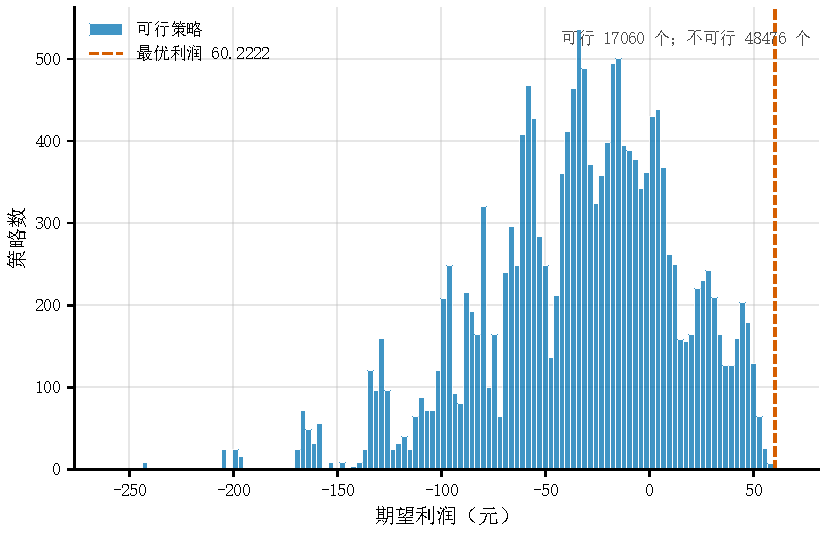
\includegraphics[width=0.96\textwidth]{../../figures/q3/fig_q3_profit_distribution.pdf}
  \caption{全枚举 65536 个策略的期望利润分布}
  \label{fig:q3-landscape}
\end{figure}

不可行策略主要来源于“拆解回流—缺陷未识别—重复装配”的闭环。例如某下级零部件实际不合格，策略允许上级不合格品拆解，却始终不检测该零部件，则该缺陷件会在拆解后重复进入装配过程，形成不含交付状态的闭合状态类，期望成本无有限解。图~\ref{fig:q3-infeasible-loop}示意该失效循环；全枚举共识别出 48476 个此类不可行策略，占全部策略的 $74\%$，而可行与不可行策略的划分仅由决策位结构决定，与具体参数取值无关（次品率大于 0 时）。

\begin{figure}[H]
  \centering
  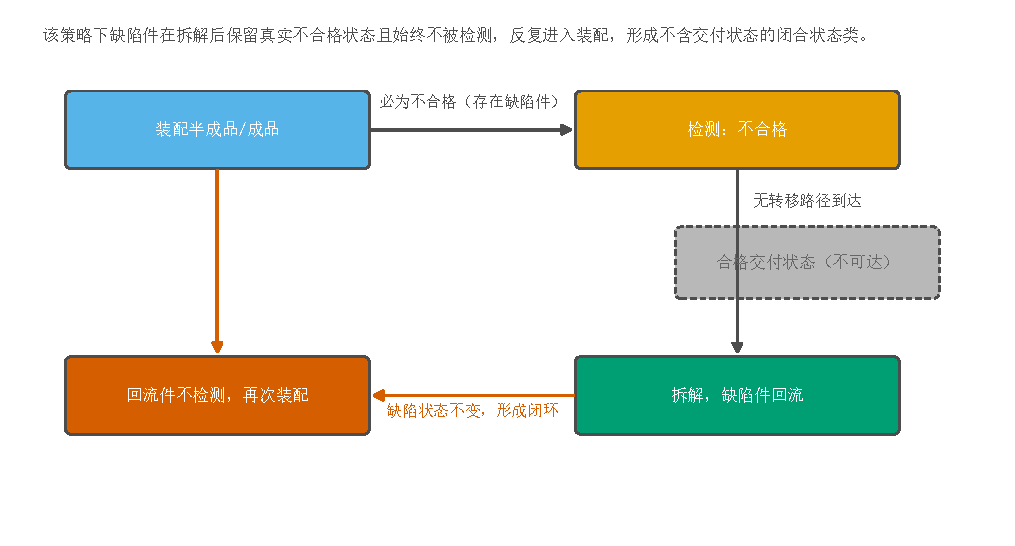
\includegraphics[width=0.86\textwidth]{../../figures/q3/fig_q3_infeasible_loop.pdf}
  \caption{缺陷回流闭环导致策略不可行的机制示意}
  \label{fig:q3-infeasible-loop}
\end{figure}

图~\ref{fig:q3-top10}比较全枚举排名前 10 的策略：最优策略比第二名高 $2.1728$ 元；第 2--8 名与最优策略的汉明距离不超过 2，第 9、10 名不超过 3，高利润策略只在少数决策位上不同。最优策略省去成品检测（$x_{15}=0$），原因是全部零配件与半成品均已检测并拆解回流，成品缺陷主要来自 $10\%$ 的装配缺陷，其调换损失 $40$ 元与拆解回流成本之和仍低于成品检测成本 $6$ 元与后续修复成本的组合；同时保留成品拆解（$x_{16}=1$），使退回成品中的合格下级组件能够回流再利用。

\begin{figure}[H]
  \centering
  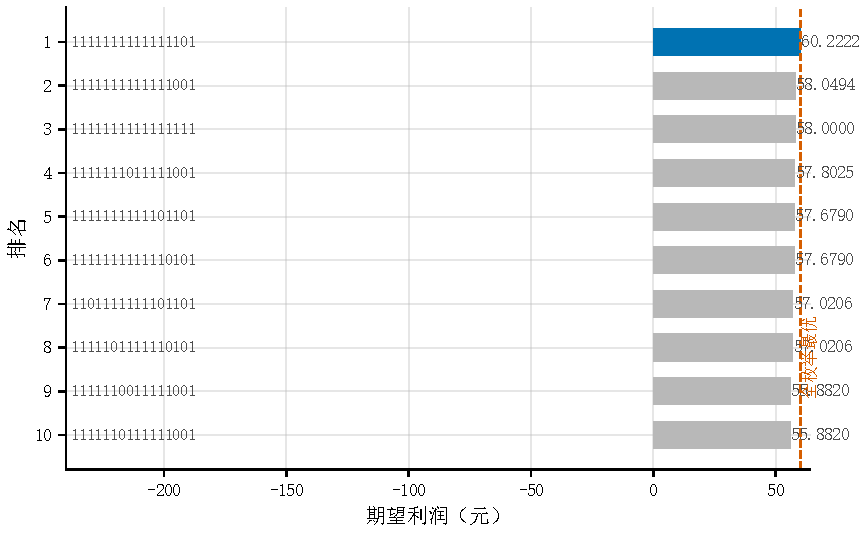
\includegraphics[width=0.90\textwidth]{../../figures/q3/fig_q3_top10.pdf}
  \caption{全枚举排名前 10 的策略期望利润比较}
  \label{fig:q3-top10}
\end{figure}

\subsubsection{遗传算法扩展性验证}

当工序或零部件数量继续增加、$2^m$ 不再可枚举时，可采用遗传算法（Genetic Algorithm，GA）\cite{ga-holland}作为启发式扩展方法：染色体为策略编码 $X$，适应度为解析期望利润 $E[\Pi(X)]$。在本题可枚举规模下，多次独立运行均复现精确枚举所得最优策略；该结果仅验证其扩展可用性，正式最优结论仍由完全枚举给出。

\subsubsection{验证与敏感性}

为检验递推实现与随机模拟的一致性，对三个代表性策略各进行 20000 次 Monte Carlo 模拟：固定策略空间内的最优策略 $1111111111111101$、近优策略 $1111111111111001$，以及含较多拆解回流环节的可行策略 $1111111111101101$。三个策略的解析期望成本 $139.7778$、$141.9506$、$142.3210$ 元分别位于对应模拟的 $95\%$ 置信区间 $[139.2744,139.9643]$、$[141.4423,142.2149]$、$[141.7859,142.5764]$ 元内，且 20000 次模拟均完成交付、无未终止样本。解析值与模拟值的差异在随机误差范围内，支持递推实现的正确性。

为检验最优策略对参数的依赖，对五类参数分别乘以 $0.8$、$1.0$、$1.2$：零配件检测成本、零配件次品率、成品次品率、调换损失与拆解成本，每次只改变一类参数，并对每个扰动点进行全策略精确枚举。结果表明，在这五类参数的 $\pm20\%$ 单因素扰动下，固定策略空间内的最优策略均保持 $1111111111111101$；每个扰动点的最优性均由该参数下的完全枚举保证。图~\ref{fig:q3-sensitivity}给出各扰动点下的最优期望利润，表~\ref{tab:q3-sensitivity}列出精确数值。

\begin{figure}[H]
  \centering
  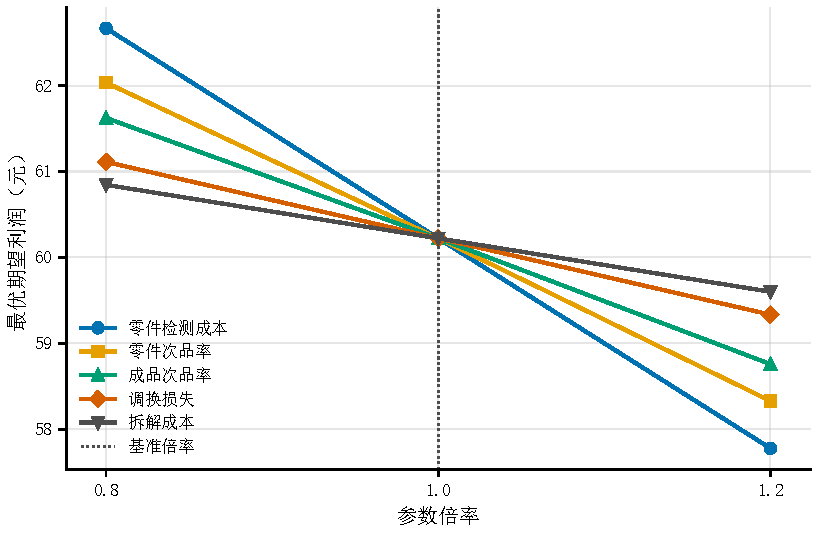
\includegraphics[width=0.96\textwidth]{../../figures/q3/fig_q3_sensitivity.pdf}
  \caption{五类参数扰动下的最优期望利润}
  \label{fig:q3-sensitivity}
\end{figure}

\begin{table}[H]
  \centering
  \caption{五类参数 $0.8/1.0/1.2$ 倍扰动下的最优期望利润（元）}
  \label{tab:q3-sensitivity}
  \begin{tabular}{lccc}
    \toprule
    参数 & $0.8$ 倍 & $1.0$ 倍 & $1.2$ 倍 \\
    \midrule
    零配件检测成本 & $62.6667$ & $60.2222$ & $57.7778$ \\
    零配件次品率 & $62.0338$ & $60.2222$ & $58.3283$ \\
    成品次品率 & $61.6232$ & $60.2222$ & $58.7576$ \\
    调换损失 & $61.1111$ & $60.2222$ & $59.3333$ \\
    拆解成本 & $60.8444$ & $60.2222$ & $59.6000$ \\
    \bottomrule
  \end{tabular}
\end{table}

利润对零配件次品率与成品次品率的变化较大：在 $\pm20\%$ 扰动范围内，两者的最大绝对利润偏差分别约为 $1.89$ 元与 $1.46$ 元；零配件检测成本上升 $20\%$ 后仍保持全部检测，说明在该参数邻域内“全检测”方案不是由检测成本临界决定的。上述结论限定在五类参数的单因素 $\pm20\%$ 网格内，不扩展到联合扰动。

\subsubsection{本问结论}

在固定策略空间内，问题三的最优决策方案为 $1111111111111101$，即全部零配件与半成品检测、不合格半成品拆解、成品不检测、不合格成品拆解，期望成本 $139.7778$ 元、期望利润 $60.2222$ 元。该结论由全策略精确枚举、Monte Carlo 置信区间检验与五类参数完全枚举敏感性三重证据支持；遗传算法复现该最优解，仅作为更大策略空间的扩展依据。
